Die Versuchsdurchführung erfolgt gemäß der Norm MIL-STD-883E. Der Messplatz befindet sich im Gebäude C12, Raum 3.28. Die verwendeten Geräte umfassen den Schertester Condor Sigma von XYZTec sowie das Mikroskop Keyence VHX 1000. Das Experiment wird in zwei Abschnitten durchgeführt: zunächst der Schertest, gefolgt von der Analyse der Bruchbilder.

\subsection{Schertest Durchführung}
Die Proben werden gemäß den Spezifikationen vorbereitet. Es werden zwei Scherprüflinge untersucht:
\begin{itemize}
    \item Scherprüfling 1: Versilberter Kupfer-Scherkörper, gesintert auf eine Kupferbodenplatte.
    \item     Scherprüfling 2: Kupfer-Scherkörper, laminiert auf eine Kupferbodenplatte.
\end{itemize}
Die Probekörper werden präzise auf der Vorrichtung des Scherprüfgeräts positioniert, sodass ausschließlich der Prüfling mit dem Schermesser in Kontakt tritt. Die Spannvorrichtung wird so justiert, dass eine parallele Ausrichtung zwischen den Kanten des Prüflings und dem Schermeißel erreicht wird, um eine gleichmäßige Kraftübertragung sicherzustellen. Zur Feinpositionierung wird ein Mikroskop verwendet.\\

Der Schermeißel wird ohne direkten Kontakt zum Prüfling in Position gebracht. Anschließend wird ein vorab programmiertes Verfahren aktiviert, bei dem der Meißel zunächst kurz die Halterung berührt und anschließend auf die definierte Höhe des Prüflings eingestellt wird, um den Schervorgang durchzuführen.\\

Die Abscherung der Prüflinge erfolgt mittels des Schermeißels, wobei die aufgebrachte Kraft kontinuierlich über den Verfahrweg des Meißels erfasst wird. Um eine hohe Reproduzierbarkeit zu gewährleisten, werden die Messungen mit zehn Prüflingen desselben Typs mehrfach wiederholt. Alle relevanten Messdaten werden in Echtzeit erfasst und mit den spezifizierten Sollwerten verglichen.\\

Nach Abschluss des Schervorgangs wird die aufgebrachte Kraft durch das Scherprüfgerät protokolliert. Anschließend erfolgt eine mikroskopische Untersuchung der Bruchstellen zur detaillierten Analyse der Bruchmuster. (siehe \hyperref[CondorSigma]{Abbildung 4})

\begin{figure}[H]
    \centering
    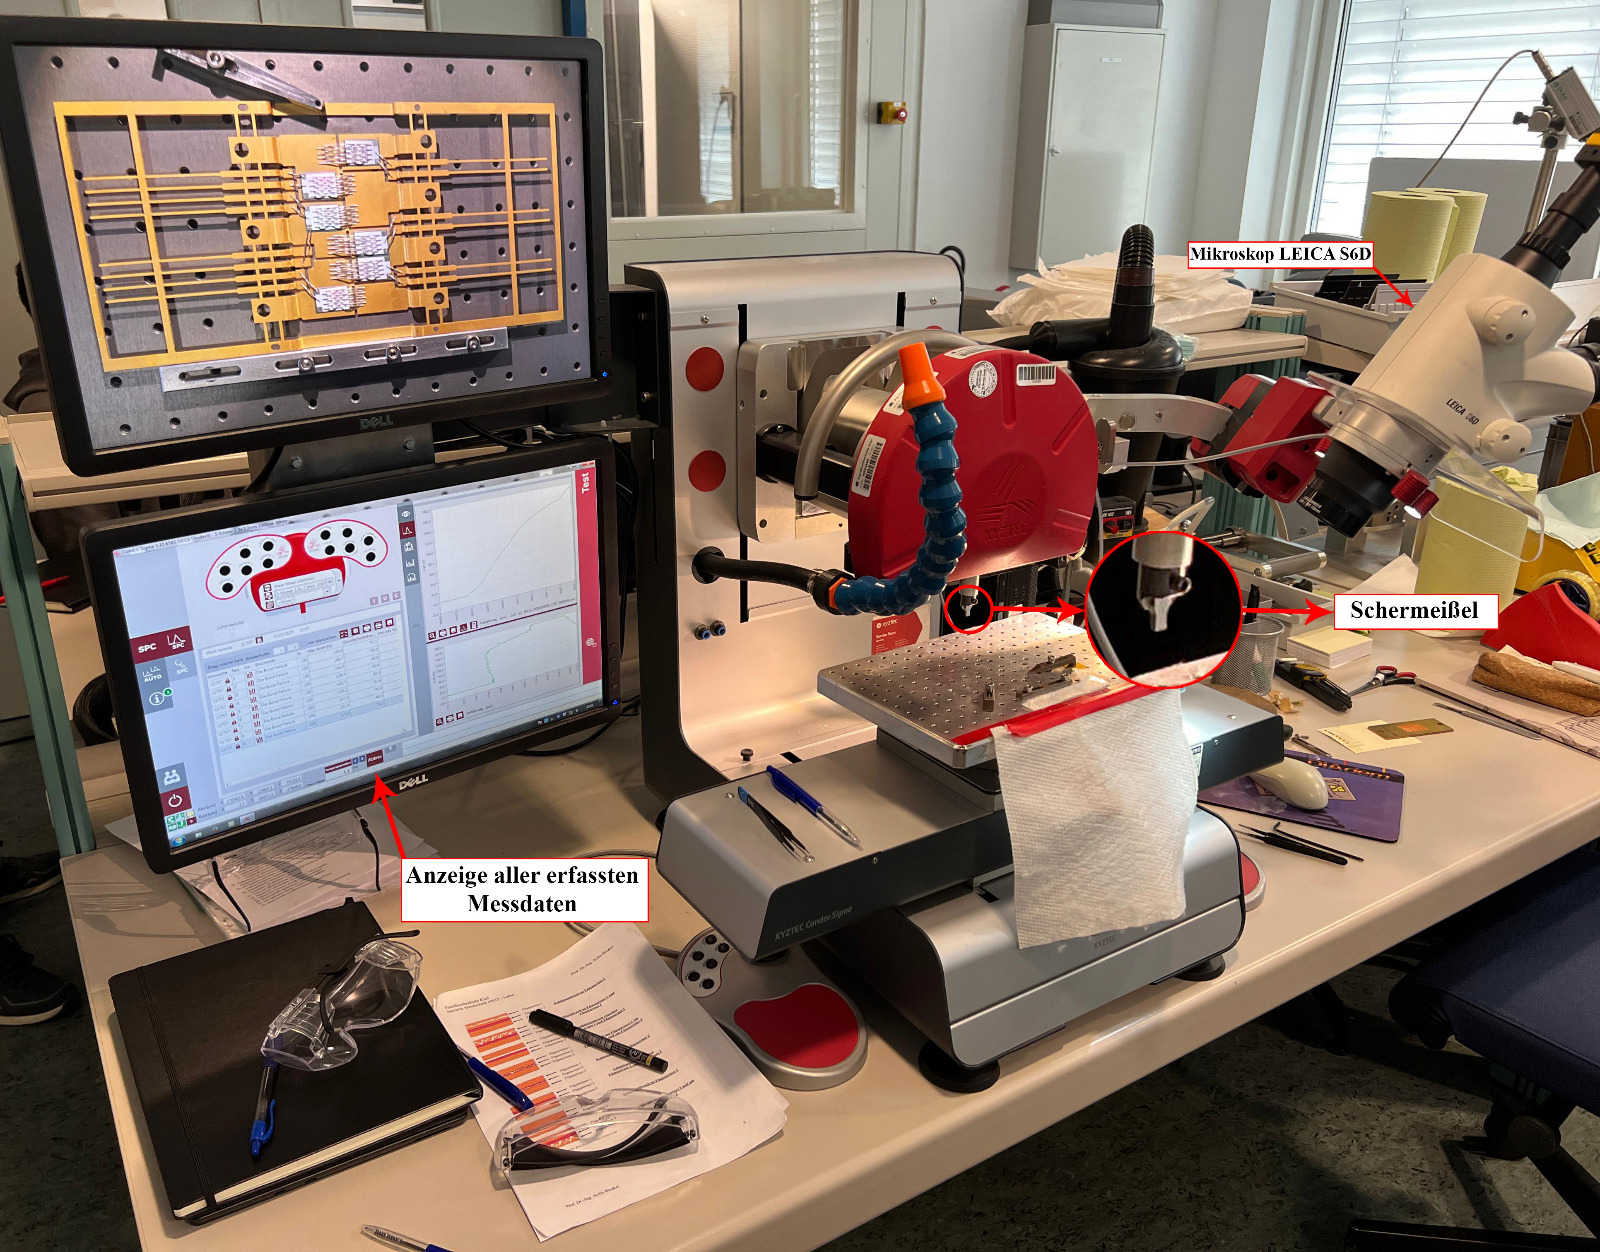
\includegraphics[scale=0.2]{Bilder/WhatsApp Image 2025-03-28 at 17.45.42.jpeg}
    \caption{Scherprüfgerät Condor Sigma der Firma XYZTec während des Prüfprozesses, (Selbsterstellte Abbildungen)}
    \label{CondorSigma}
\end{figure}

\subsection{Analyse der Bruchbilder}
Zur Analyse der Bruchbilder wird das digitale Mikroskop Keyence VHX-1000 verwendet. Die Kupfer-Scherkörper werden auf einer Kupferbodenplatte unter das Mikroskop gelegt, wobei Fokus und Vergrößerung manuell justiert werden. Nach der Untersuchung der Prüfkörper wird die Kupferbodenplatte analysiert, um die Art des Bruchs zu identifizieren. Dabei werden sowohl duktile als auch spröde Bruchmerkmale dokumentiert und klassifiziert. (siehe \hyperref[VHX]{Abbildung 5})

\begin{figure}[H]
    \centering
    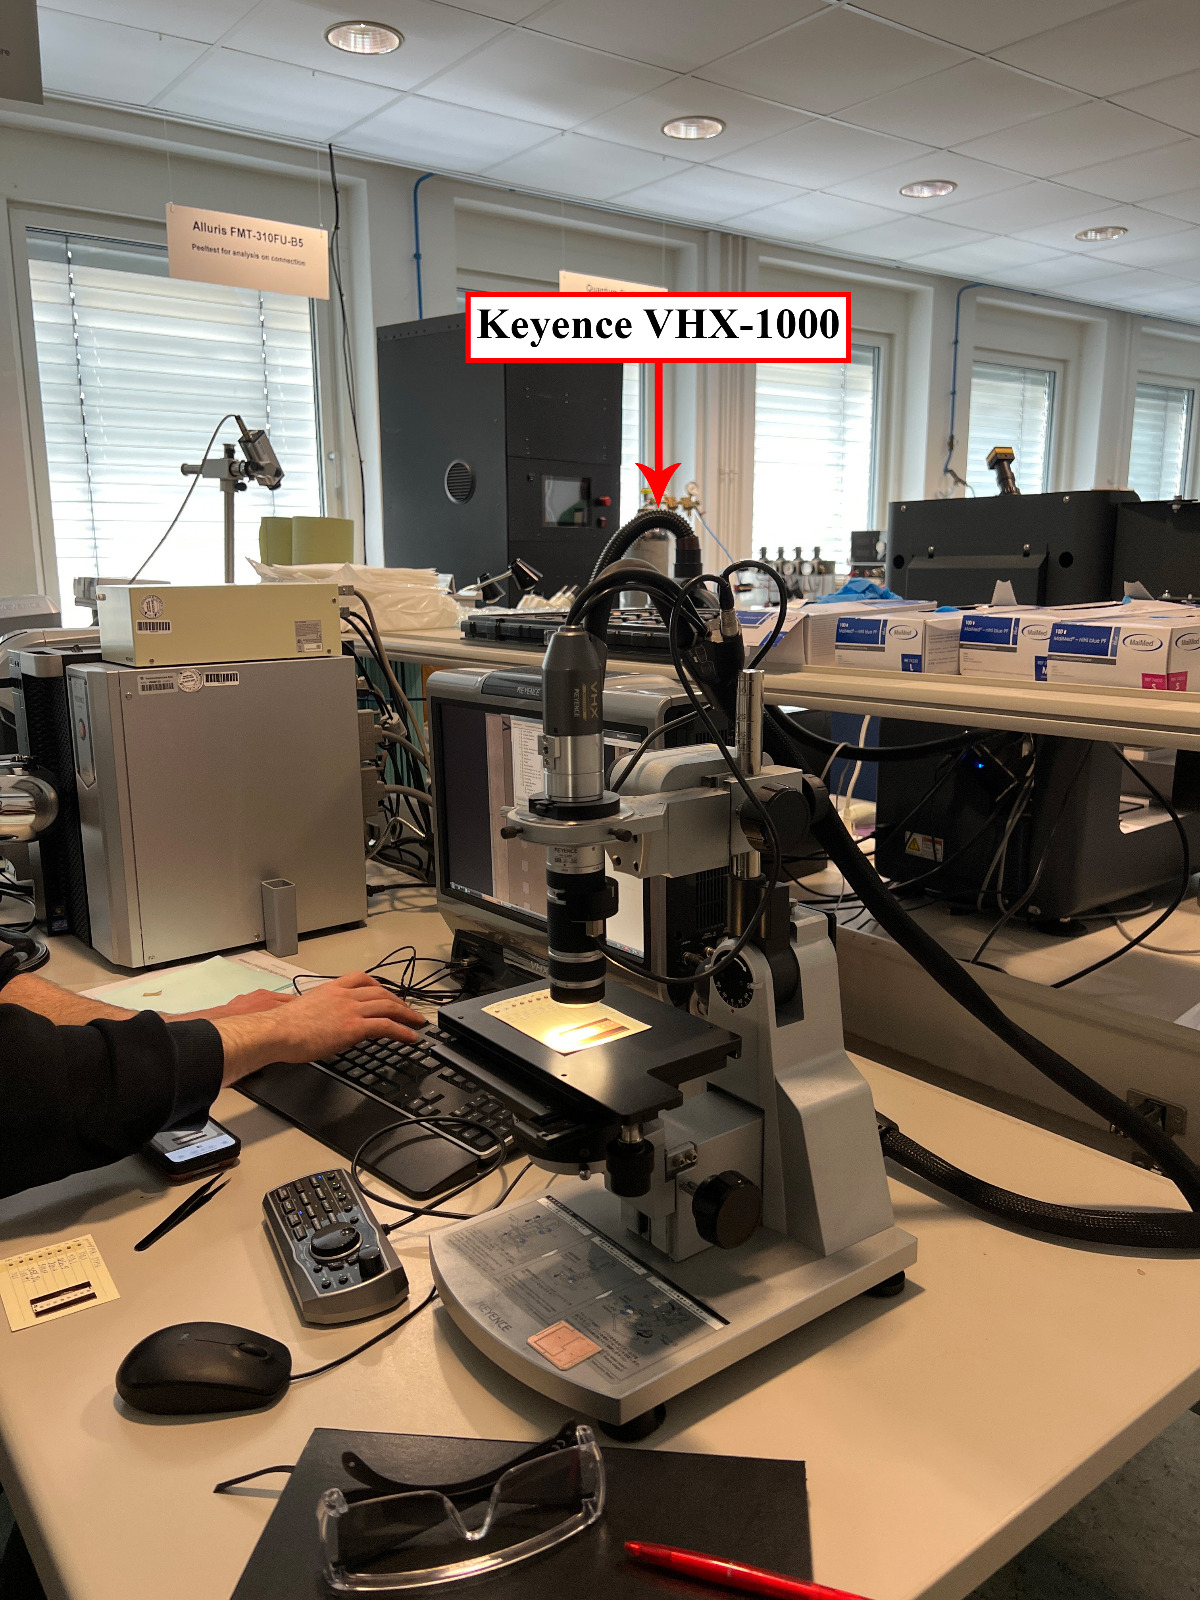
\includegraphics[scale=0.2]{Bilder/WhatsApp Image 2025-03-28 at 20.46.08.jpeg}
    \caption{Mikroskop Keyence VHX-1000 zur Bruchbildanalyse, (Selbsterstellte Abbildungen)}
    \label{VHX}
\end{figure}